\chapter{Heat Equation -- 2D -- Active and Passive elements}

\modinfo{Directory}{PassiveElements}
\modinfo{Solvers}{\Idx{HeatSolve}}
\modinfo{Tools}{\Idx{ElmerGUI}}
\modinfo{Dimensions}{2D,Transient}
\modinfo{Author}{original author not known}

\subsection*{Case definition}

This tutorial shows an example of using \Idx{passive elements} in Elmer. This feature allows the activation and deactivation of parts of the geometry during the simulation. This tutorial uses the heat equation solver to demonstrate this capability. Use with other solvers is analogous.

The geometry of the problem consists of two parts. The lower edge of the lower part is held at constant temperature of 1 degrees. The upper body is heated with a constant heating power. Between time steps 5 and 6 the two bodies are connected by two heat conductors, and the heat is conducted from the higher body to the lower one. The goal of the simulation is to model the temperature distribution in the system over time. 

The problem is a pure heat transfer problem that may be solved with \texttt{HeatSolve}. 

The geometry for this tutorial looks like as shown in figure \ref{fg:geometry}.

\begin{figure}[H]
\centering
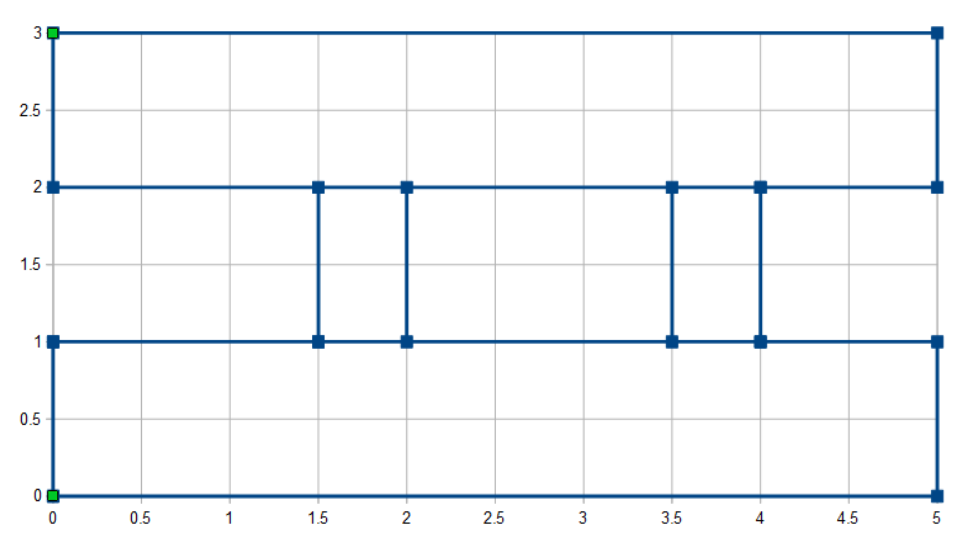
\includegraphics[width=0.8\textwidth]{geometry.png}
\caption{Geometry}\label{fg:geometry}
\end{figure}  

\subsection*{ElmerGUI Equation Menu}

We will be using the \Idx{Heat Solver}, which is one of the default, pre-loaded GUI definitions, so it does not need to be manually activated.  For reference, the  \texttt{\Idx{heatequation.xml}} definition file is, by default, located in Linux in:

\texttt{\$ELMER\_HOME/share/ElmerGUI/edf}

\noindent and in Windows, located in:

\texttt{C:/Program Files/Elmer 9.0-Release/share/ElmerGUI/edf}\\


\subsection*{Solution procedure}

The mesh is given in ElmerGrid format in file \texttt{tmesh.grd}, load this file.

\ttbegin
File 
  Open -> tmesh.grd
\ttend

You should obtain your mesh and may check \texttt{Model Summary...} that it consists of 2018 surface elements.  Your mesh should look like as shown in figure \ref{fg:mesh}

\begin{figure}[H]
\centering
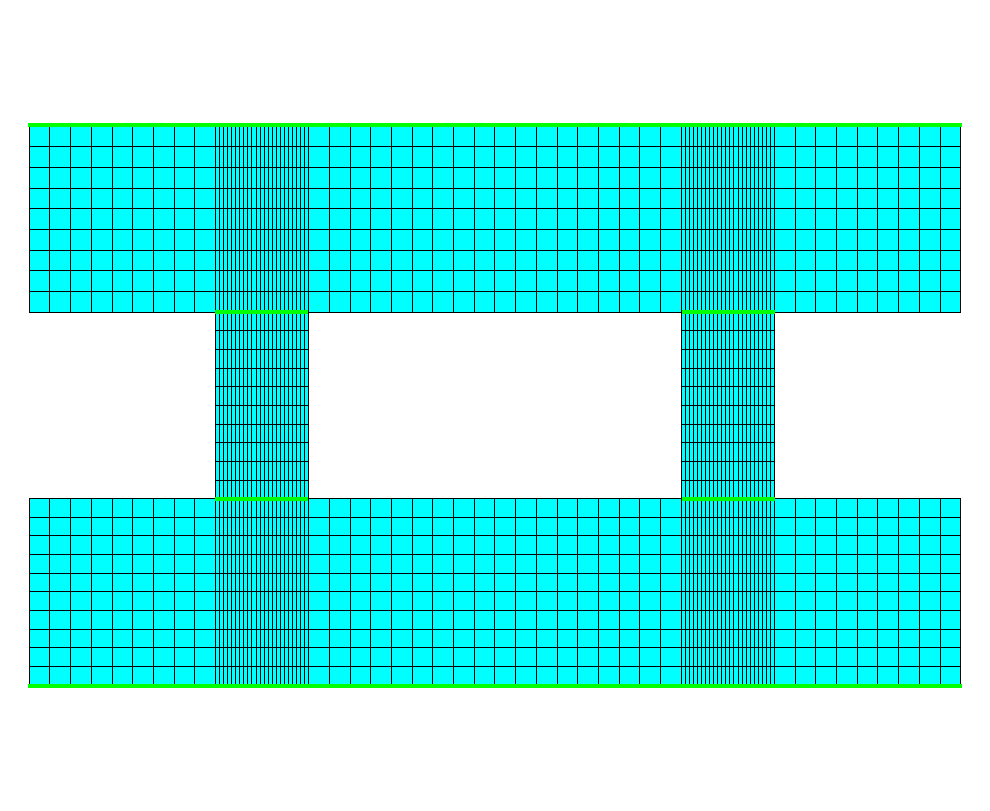
\includegraphics[width=0.8\textwidth]{mesh}
\caption{Mesh}\label{fg:mesh}
\end{figure}

After we have the mesh we start to go through the Model menu from the top to bottom.  In the Setup we choose things related to the whole simulation such as file names, time stepping, constants etc.  

The simulation is carried out in 2-dimensional Cartesian coordinates.

2nd order bdf time stepping method is selected with 15 steps and with step size of 1 seconds.

The heat equation is solved with an iterative method. The system is linear, thus multiple non-linear iterations are not needed.

\ttbegin
Model
  Setup 
    Simulation Type = Transient
    Steady state max. iter = 1
    Time Step Intervals = 15
    Time Step Sizes = 1
  Apply
\ttend

In the equation section we choose the relevant equations and parameters related to their solution. 

In this case we'll have one equation (named ``Heat'') which consists of the heat equation.

When defining Equations and Materials it is possible to assign to the bodies immediately, or to use mouse selection to assign them later. In this case we have just three bodies and therefore its easier to assign the Equation and Material to it directly. 

For the linear system solvers we are happy to use the defaults. One may however, try out different preconditioners (ILU1,\ldots) or direct Umfpack solver, for example.

\ttbegin
Model
  Equation
   Name = Heat
    Apply to Bodies = 1 2 3
    Heat Equation
      Active = on
    Add 
    OK
\ttend        
The Material section includes all the material parameters. They are divided into generic parameters which are direct properties of the material without making any assumptions on the physical model, such as the mass. Other properties assume a physical law, such as conductivities and viscosity. 

The material properties of the system are artificial. The following three properties are needed for each material.

\ttbegin
Model
  Material
    Apply to Bodies = 1 3 
    General 
      Density = 1
      Heat Capacity = 1
    Heat Equation
      Heat Conductivity = 1
    Add
    OK

  Material
    Apply to Bodies = 2
    General 
      Density = 1
      Heat Capacity = 10
    Heat Equation
      Heat Conductivity = 1
    Add
    OK
\ttend

A Body Force represents the right-hand-side of a equation. It is generally not a required field for a body. 

There are three bodies with the same equation but different material properties. Body 3 is heated by a constant body force. Body 2 forms the connecting parts of the system. An initial condition as well as a body force is defined for this body. The body force contains the initial deactivation, and later activation, of the connecting part. Note that this part is included in the geometry all the time, but the passive command is used to define when they are included into the simulation.

Now the passive condition for the connecting part is defined. When the parameter  \texttt{Temperature Passive} has a value larger than zero, the current element is excluded from the solution, otherwise it is included as a normal element. The parameter may depend on variables, coordinates or time. Here it is defined to depend on time using a tabular format.

The section `Free text input' is used, because the option to define a passive element has not been added to the ElmerGUI menu file `heatequation.xml'.  For any solver, one can always add additional commands by using the Free text input box.

\ttbegin
Model
  Body Force
    Name = Heat Source
    Apply to Bodies = 3
    Heat Equation
       Volume Sources
         Heat source = 10
    Add 
    OK

  Body Force
    Name = Passive
    Apply to Bodies = 2
    Heat Equation
       Free text input
         Temperature Passive = Variable time
            Real
              0.0     1.0
              5.0     1.0
              5.2    -1.0
              8.0    -1.0
           End
    Add 
    OK
\ttend    

Initial conditions should be given to transient cases, and probably are not needed for steady state solutions. 

In this case we choose a constant Temperature for the passive element.  The initial condition for the initially passive elements is taken to be 5 degrees; a temperature halfway between the colder part and the hotter part of the system.
 
\ttbegin
Model
  Initial Condition 
    Name = Initial Guess
    Apply to Bodies = 2
    Heat Equation
      Temperature = 5.0
    Add 
    OK
\ttend

Only one boundary condition may be applied to each boundary and therefore all the different physical BCs for a boundary should be grouped together. 

The boundary conditions are simple. The lower boundary of the lower body is held at 1 degrees and the upper boundary of the upper body at 10 degrees.  The side walls are assumed to be adiabatic.

\ttbegin
Model
  Boundary Condition
    Name = Bottom
    Heat Equation
      Temperature = 1.0
    Add
    New

  Boundary Condition
    Name = Top
    Heat Equation
      Temperature = 10.0
    Add
   OK 
\ttend   

The conditions may also be assigned to boundaries in the Boundary condition menu, or by clicking on each boundary with the mouse. Here we use the latter approach as that spares us of the need to know the indexes of each boundary.

\ttbegin
Model
  Set boundary properties
    Choose Bottom -> set boundary condition Bottom
    Choose Top -> set boundary condition Top
   OK 
\ttend

For the execution ElmerSolver needs the mesh files and the command file.  We have now basically defined all the information for ElmerGUI to write the command file. After writing it we may also visually inspect the command file.
\ttbegin
Sif 
  Generate
  Edit -> look how your command file came out  
\ttend

Before we can execute the solver we should save the files in a directory.  The ElmerGUI project includes all the files needed to restart the case.

\ttbegin
File 
  Save Project
\ttend

After we have successfully saved the files we may start the solver.

\ttbegin
Run
  Start solver
\ttend

A convergence view automatically pops up showing relative changes of each iteration.

When there are some results to view we may start the postprocessor also.

\ttbegin
Run
  Start ParaView
\ttend

\subsection*{Results}

Due to the number of the time steps the simulation may take around 15 seconds.\\

You may inspect the results with Paraview or with ElmerVTK.\\

In Figure \ref{fg:temp} the obtained temperature distribution is presented, where the left image shows the passive condition, and the right image shows the active condition. 

\begin{figure}[h]
\centering
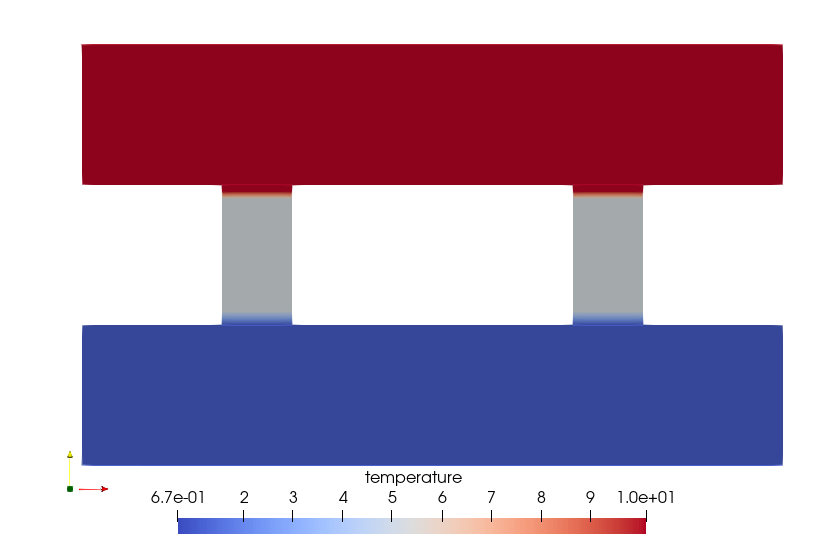
\includegraphics[width=0.48\textwidth]{temp-4}
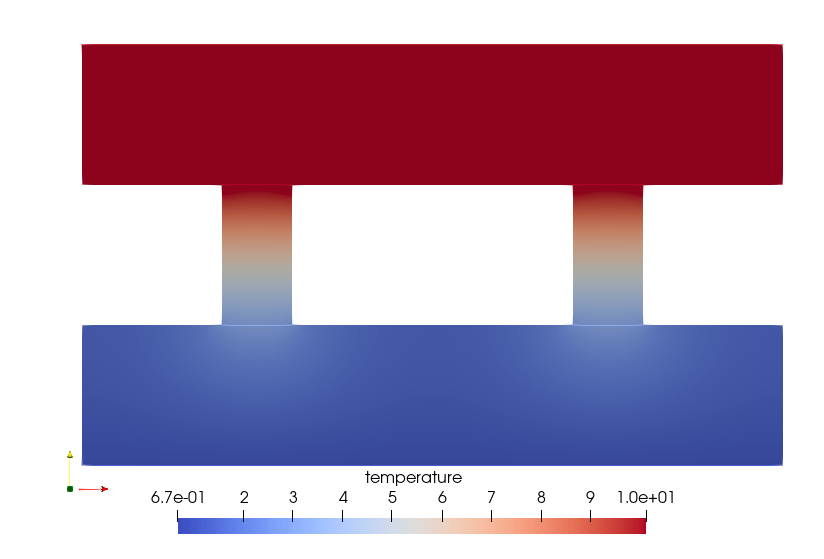
\includegraphics[width=0.48\textwidth]{temp-6}
\caption{Temperature distribution at 4 and 6 seconds}\label{fg:temp}
\end{figure} 

\hfill
